\documentclass{article}
\usepackage{cite}

\usepackage{titlesec}
\setcounter{secnumdepth}{4}

\usepackage{amsmath}
\usepackage{caption}
\usepackage{graphicx}
\graphicspath{{./figures/}}

\title{Data Analysis for Predictive Maintenance of a Straightening Machine in the Steel Industry}
\date{2023-XX-XX}
\author{Paul Barron}
\begin{document}
\pagenumbering{gobble}
\maketitle
\newpage
\pagenumbering{arabic}
\tableofcontents
\newpage
\section{Abstract}
 
\newpage
\section{Introduction}

Understand what signals are related to each other
Understand signals from a statistical point of view
Identify which features are the important ones and which are not of interest

\newpage  
\section{Literature Review}
\subsection{Condition Monitoring}
Condition monitoring.\\
Reference ~\cite{caesarendra2017review}.\\
Reference ~\cite{james2013introduction}.\\
Reference ~\cite{soualhi2021novel}.
"We tend to select statistical learning methods on the basis of whether
the response is quantitative or qualitative; i.e. we might use linear regression when quantitative and logistic regression when qualitative." From textbook.
\subsection{Straightening Machine}
\newpage  
\section{Methodology}
Preprocessing: you could standardize the signals, eliminate the dc-offset, … before calculating the features.
Calculate features of the different signals, i.e., correlations between raw signals, kurtosis, mean, skewness, …,
Verify features which are extracted from the diagnostic feature extraction toolbox, i.e., what it is kurtosis, THD,… for the toolbox. You can compare the results given by the matlab function and the toolbox. Important to look at the formula which is given on the help description of the function.

Compute correlations between 2 features.
Calculate a in X1 = aX2, where X1 and X2 represents the features.
Calculate R2, which relates to the variance in linear regression models.
Plot some of the regression models between 2 features which are highly correlated where X1 is one axis, and X2 is the other axis. Do not plot all of them.

Compute a multivariable regression model.
Guide yourself by eliminating features which are highly correlated between each other by using the info you got in the previous part where you compute correlations between 2 features.

\subsection{Description of Data}
The data used for this analysis consists of an hour of operational data for 15 days. I do now know whether it was taken from the same time each day. The assumption is that the file name corresponds with the data that the data was taken.
The file names are given in \ref{fileNames}.
\begin{center}
\begin{tabular}{ |l| } 
 \hline
 B\_30\_03.mat \\
 \hline 
 B\_31\_03.mat \\
 \hline 
 B\_01\_04.mat \\
 \hline 
 B\_02\_04.mat \\
 \hline
 B\_03\_04.mat \\
 \hline 
 B\_04\_04.mat \\
 \hline 
 B\_05\_04.mat \\
 \hline
 B\_06\_04.mat \\
 \hline 
 B\_07\_04.mat \\
 \hline 
 B\_08\_04.mat \\
 \hline 
 B\_09\_04.mat \\
 \hline 
 B\_10\_04.mat \\
 \hline
 B\_11\_04.mat \\
 \hline 
 B\_12\_04.mat \\
 \hline
 B\_13\_04.mat \\
 \hline
\end{tabular}
\captionof{table}{File names which indicate the day the data was taken}\label{fileNames}
\end{center}

The list of signals given be the company are given in Table \ref{signalNames}.
\begin{center}
\begin{tabular}{ |c|l| }
 \hline
 Signal Number & Signal Name \\ 
 \hline
21:07 & Angle over Rolls (degrees) \\
 \hline
21:10 & Position over Rolls (mm) \\
 \hline
21:12 & Actual moment over Rolls (Nm) \\
 \hline
21:17 & Angle under roll (degrees) \\
 \hline
21:20 & Actual moment under Rolls (Nm) \\
 \hline
21:28 & Vibration measurements (mm per s) \\ 
 \hline              
21:31 & Width position (mm) \\
 \hline
21:32 & Height position (mm) \\
 \hline
21:33 & Error position for height (mm) \\
 \hline
21:34 & Error position for the width (mm) \\
 \hline
21:35 & Set point force (KN) \\
 \hline
21:36 & Actual force (KN) \\
 \hline
\end{tabular}
\captionof{table}{Signal Names}\label{signalNames}
\end{center}

Figure \ref{fig:SignalTrace21.20} shows 21:20 Actual moment under Rolls (Nm)

\begin{figure}[!ht]
    \centering
    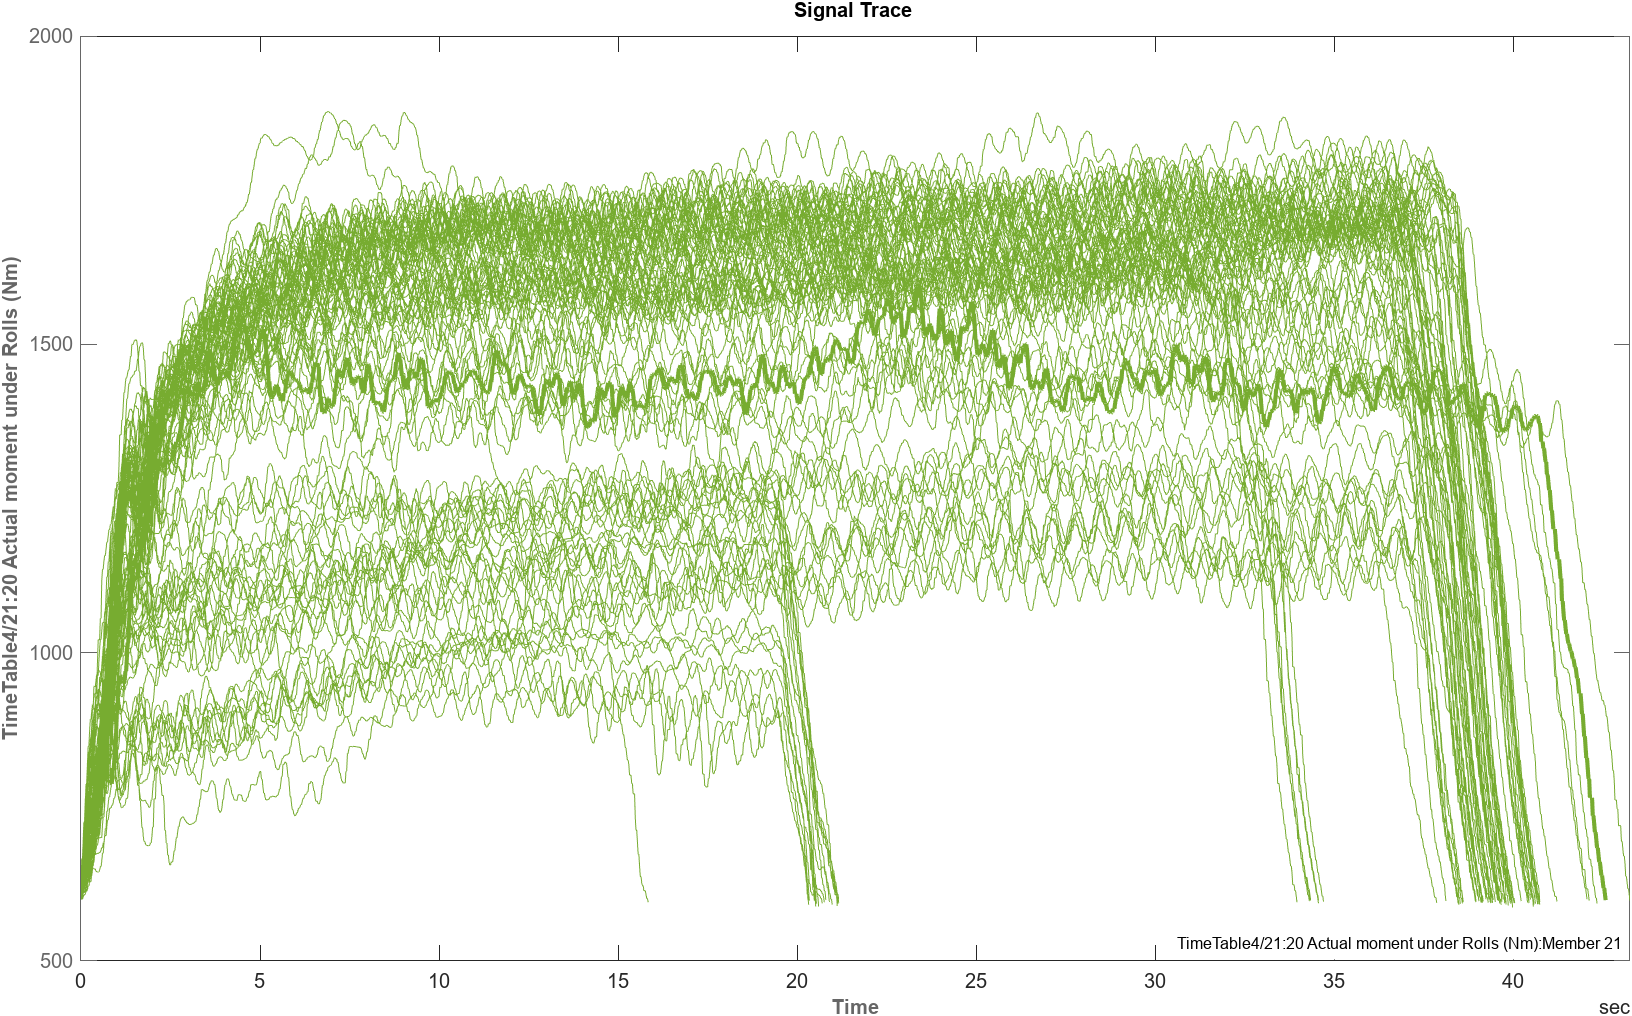
\includegraphics[width=\textwidth, height=\textheight, keepaspectratio]{figures/SignalTrace21.20.png}
    \caption{SignalTrace21.20}
    \label{fig:SignalTrace21.20}
\end{figure}

Figure \ref{fig:SignalTrace21.12} shows ...
\begin{figure}[!ht]
    \centering
    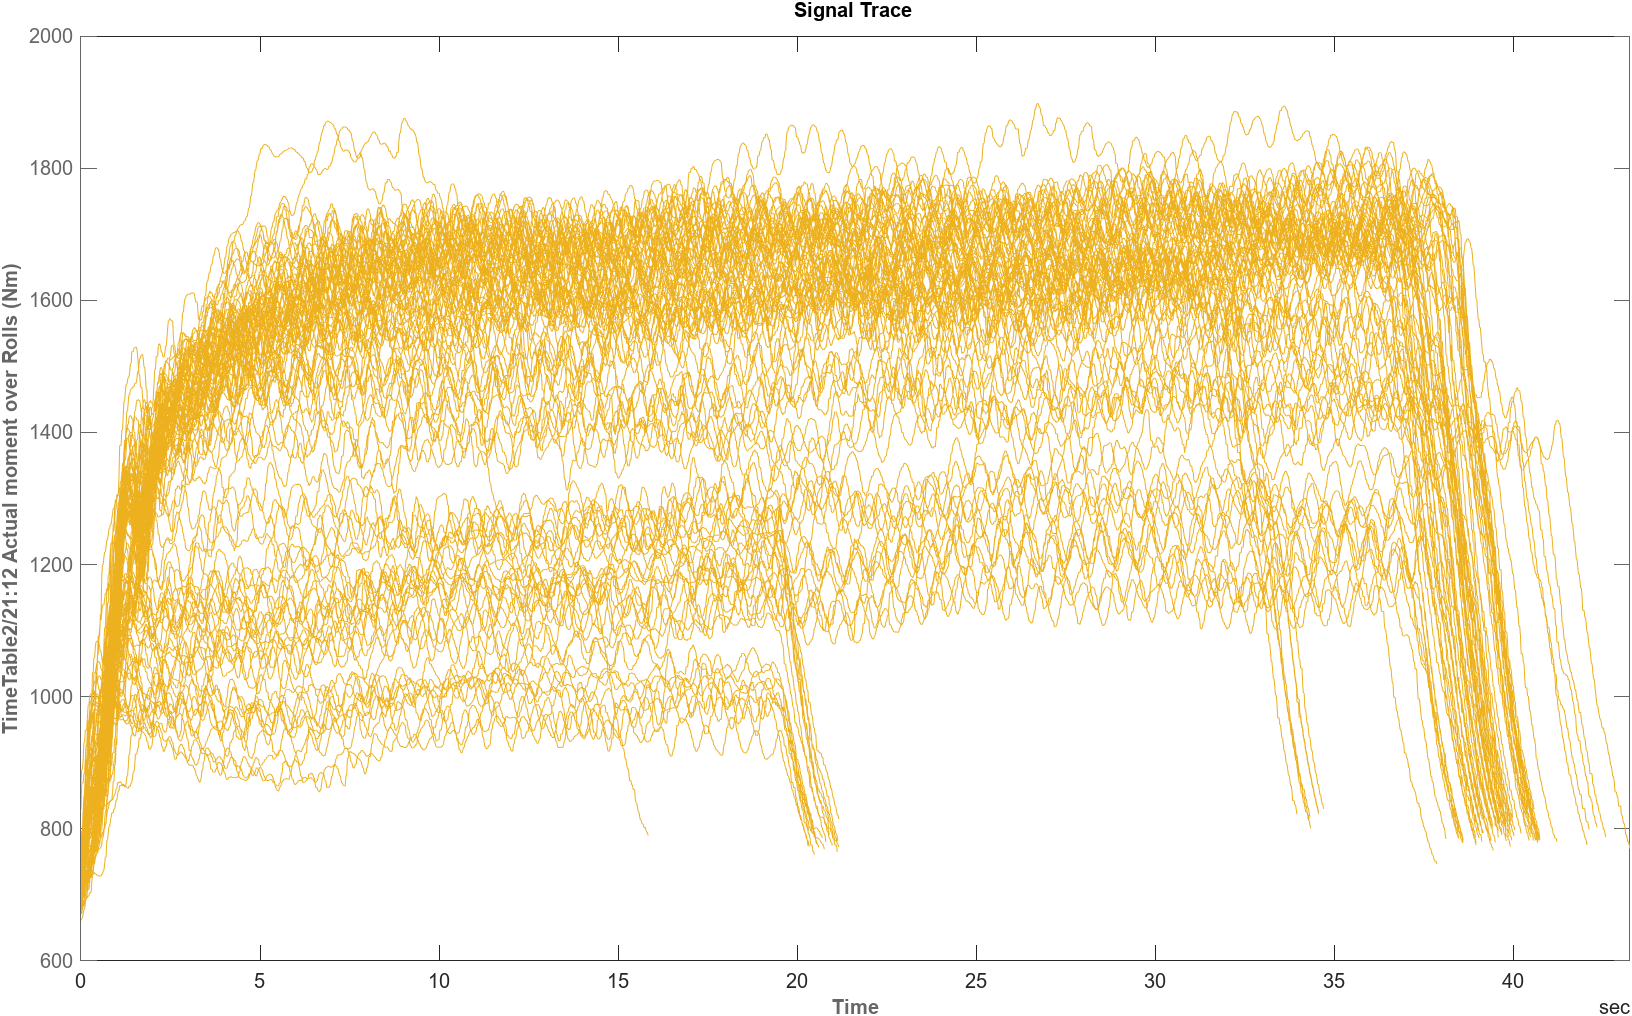
\includegraphics[width=\textwidth, height=\textheight, keepaspectratio]{figures/SignalTrace21.12.png}
    \caption{SignalTrace21.12}
    \label{fig:SignalTrace21.12}
\end{figure}

Figure \ref{fig:SignalTrace21.28} shows ...
\begin{figure}[!ht]
    \centering
    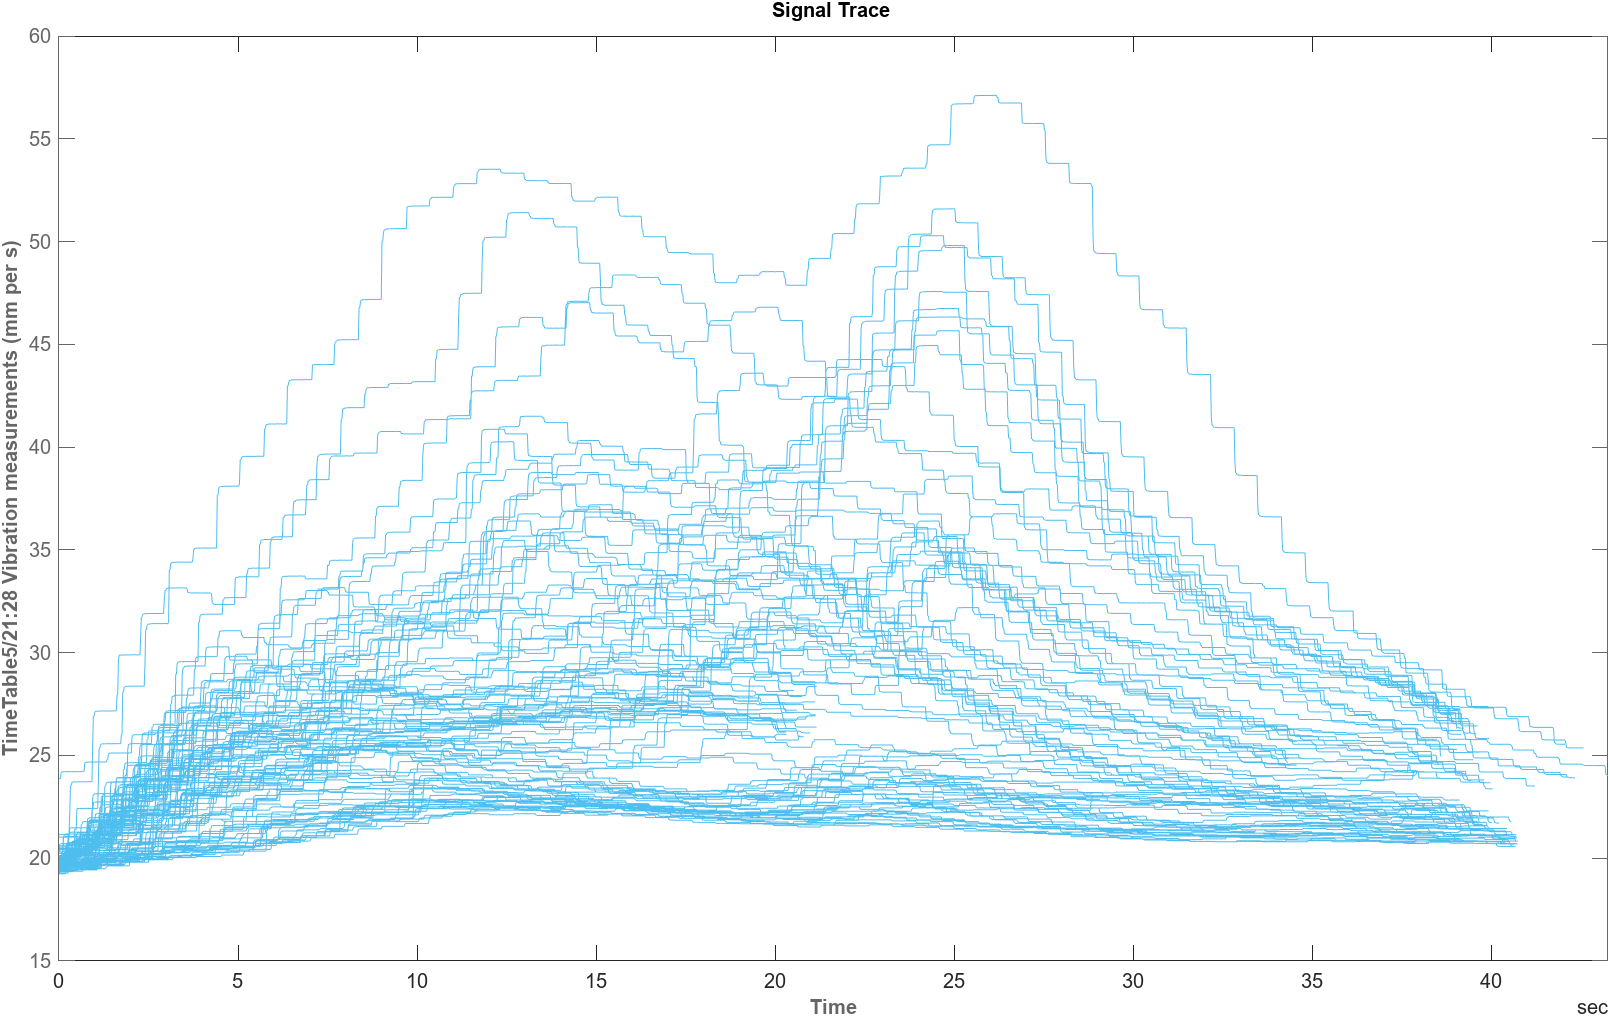
\includegraphics[width=\textwidth, height=\textheight, keepaspectratio]{figures/SignalTrace21.28.png}
    \caption{SignalTrace21.28}
    \label{fig:SignalTrace21.28}
\end{figure}

Figure \ref{fig:SignalTrace21.35} shows ...
\begin{figure}[!ht]
    \centering
    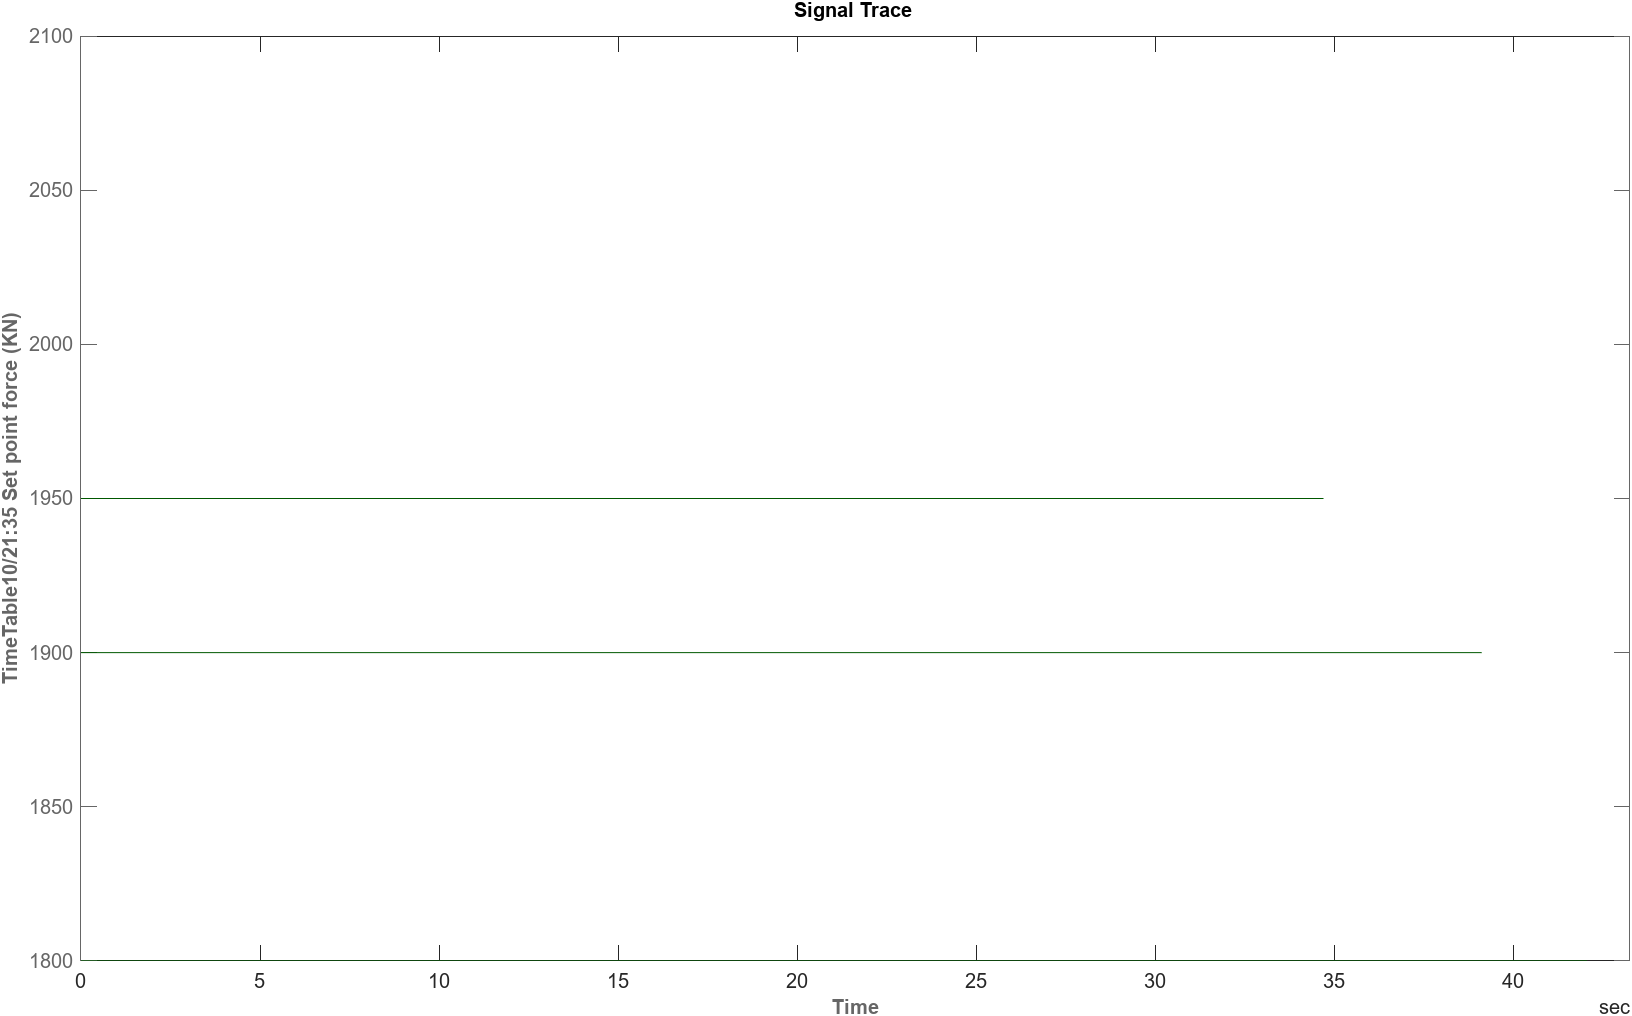
\includegraphics[width=\textwidth, height=\textheight, keepaspectratio]{figures/SignalTrace21.35.png}
    \caption{SignalTrace21.35}
    \label{fig:SignalTrace21.35}
\end{figure}
\subsection{Pre-processing sand State detection}
The state detection for this application will be performed using one signal in particular./n
Discuss how many pulses were identified and how many were ruled out by being too short./n
Some of the files contained no pulses at all, B\_30\_03 and B\_04\_04, which means they contribute nothing to this analysis.
Of the remaining 13(?) files 240 pulses were identified using script/function xx./n
When looking at these 240 pulses a number of them are too short and deemed to be false pulses so a threshold of XXs is used to only retain pulses that we think are legitimate pulses.
If we remove the mean from some of the signals we are left with nothing, since some of the signals are straight lines.
\subsection{Feature Extraction}
Blah
\subsection{Statistical analysis}
$$ AIC = 2k - 2Ln(L) $$  
$$ nAIC = log $$
\subsection{Time Domain Features} 	
Features in the time domain.
\subsection{Statistical Features}
\subsubsection{Mean}
$$ \bar{x} = \frac{\sum^N_{i=i} x_i}{N} $$
\subsubsection{Standard Deviation}  
$$ Var =\frac{\sum^N_{i=1}(x_i-m)^2}{(N-1)\sigma^2} $$
\subsubsection{Root Mean Square (RMS)}
$$ RMS = \sqrt{\frac{1}{N} \sum^N_{i=1}x^2_i} $$
\subsubsection{Shape Factor}
$$ \frac{ \sqrt{\frac{1}{N} \sum^N_{i=1}x_i^2} }  {\frac{1}{N}\sum^N_{i=1}|x_i|} $$
\subsubsection{Kurtosis} 
$$ Ku = \frac{\sum^N_{i=1}(x_i-m)^4)}{(N-1)\sigma^4} $$ 
\subsubsection{Skewness} 
$$ Sk = \frac{\sum^2_{i=1}(x_i-m)^3}{(N-1)\sigma^3} $$
  
\subsection{Impulsive Metrics}  
\subsubsection{Peak Value}
$$ PV = max(x_i) $$ 
\subsubsection{Impulse Factor} 
$$ x_{clear} = \frac{x_p}{(\frac{1}{N}\sum^N_{i=1}|x_i|)} $$  
\subsubsection{Crest Factor} 
$$ CF = \frac{max|x_i|}{\sqrt{\frac{1}{N}}\sum^N_{i=1}x^2_i} $$
\subsubsection{Clearance Factor} 
$$ x_{clear} = \frac{x_p}{(\frac{1}{N}\sum^N_{i=1}\sqrt{|x_i|)^2}} $$
  
\subsubsection{Signal Processing Metrics}
\subsubsection{Signal to Noise Ratio (SNR)} 
\subsubsection{Signal-to-Noise And Distortion (SINAD)} 
\subsubsection{Total Harmonic Distortion (THD)}   

\subsubsection{Frequency Domain Features}
Features in the frequency domain.
\subsubsection{Band Power}
\subsubsection{Peak Amplitude}
\subsubsection{Peak Frequency}
\subsubsection{Best Subset Selection}

\newpage  
\section{Results}
Add some plots from the DFD of all pulses and comment on the shape of them all.
Signal 21.07 Angle over Rolls and 21.XX, 21.31, etc are fairly unexciting. They are just straight lines.
Where as signal XX.XX contains a lot of information.

21.35 is a constant signal so when we remove the mean all signals are exactly the same.

Figure \ref{fig:StateDetection} shows the pulses that were identified for from each file. Two files contained no identified pulses. In total 240(?) pulses were identified to extract features from in the next stage.

\begin{figure}[!ht]
    \centering
    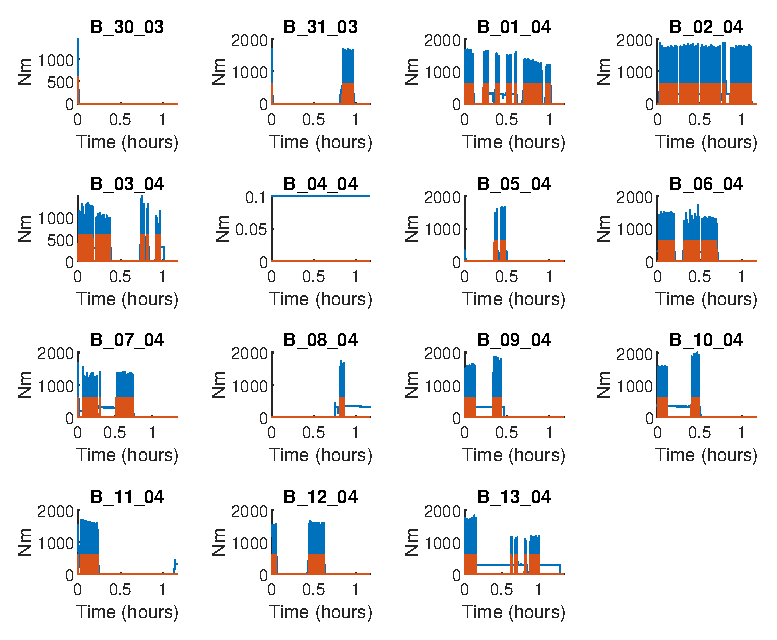
\includegraphics[width=\textwidth, height=\textheight, keepaspectratio]{figures/StateDetectionFig.eps}
    \caption{State detection signal vs 21:20 Actual moment under Rollers}
    \label{fig:StateDetection}
\end{figure}

\begin{figure}[!ht]
    \centering
    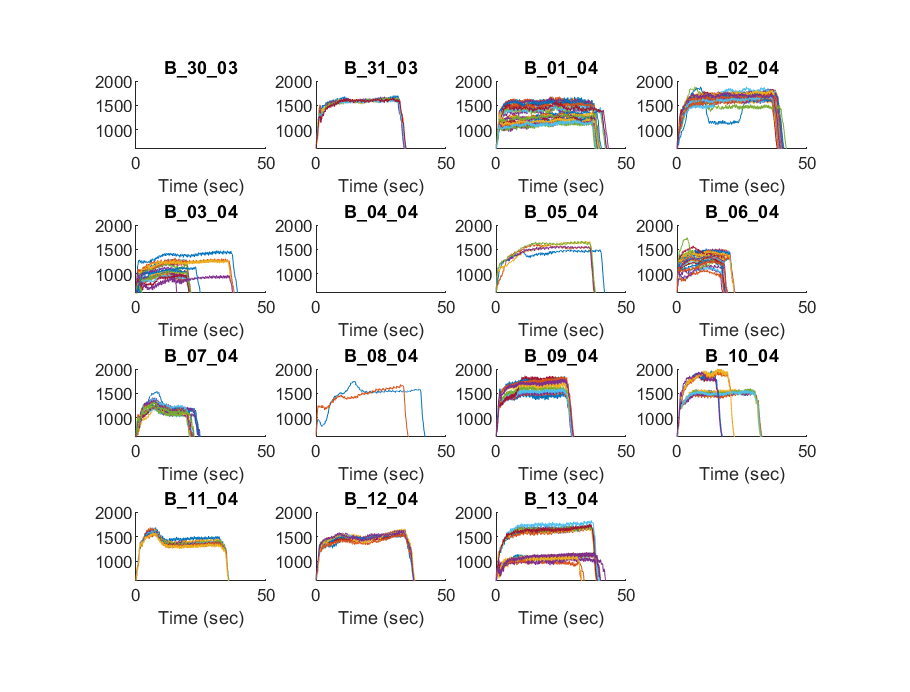
\includegraphics[width=\textwidth, height=\textheight, keepaspectratio]{figures/IdentifiedPulsesFig.eps}
    \caption{XXX}
    \label{fig:IdentifiedPulses}
\end{figure}

\newpage  
\section{Conclusion}
- We are doing inference and not prediciton
- One conlcusion could be that "for future condition monitoring work we need to only focus on this data (might only be 10%)".
- Another conclusion could be that we need to go forward to doing this and that.
- Conclusion could be what we say to the company or what we need.
\newpage 
\section{Discussion} 

\newpage  
\section{References} 
\bibliography{References}
\bibliographystyle{plain} 

\newpage  
\section{Appendix A}

\end{document}